\cite{AIShackSobelLaplacian}

Figure \ref{fig:sobel_sample_edge} shows an example of the intensity change of an image. There is a steep slope when the image changes from dark to light which means there is most likely an edge present. If the first derivative at each point is taken then the algorithm can search for a peak above some threshold and mark that point as an edge. A second derivative could be taken to find a zero crossing to signify the location of an edge and this technique is called the \emph{Laplacian edge detector} (versus the \emph{Sobel edge detector} here) and is shown in 

\begin{figure}[ht!]
{
\centering
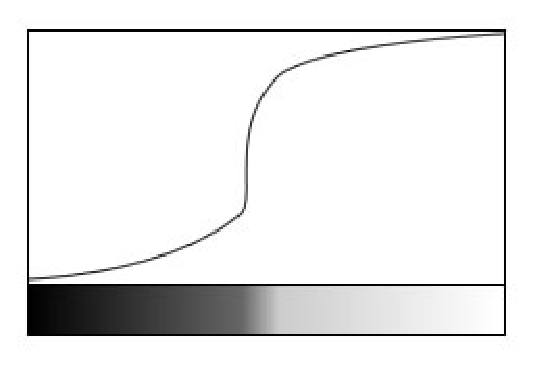
\includegraphics[width=0.5\textwidth]{eps_pics/sample-edge}
\caption{Curve representing intensity}
\label{fig:sobel_sample_edge}
}
\end{figure}

\begin{figure}[ht!]
{
\centering
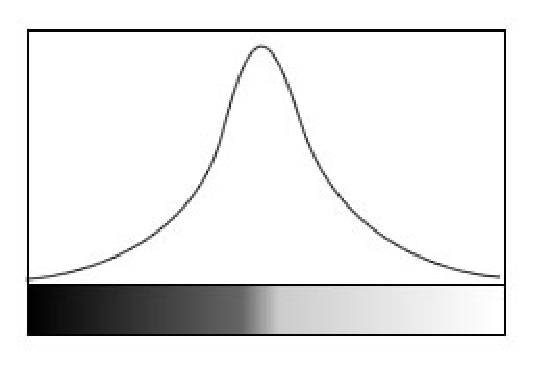
\includegraphics[width=0.5\textwidth]{eps_pics/sample-edge-first-derivative}
\caption{First derivative of the curve in Figure \ref{fig:sobel_sample_edge}}
\label{fig:sobel_sample_edge_first_deriv}
}
\end{figure}

\begin{figure}[ht!]
{
\centering
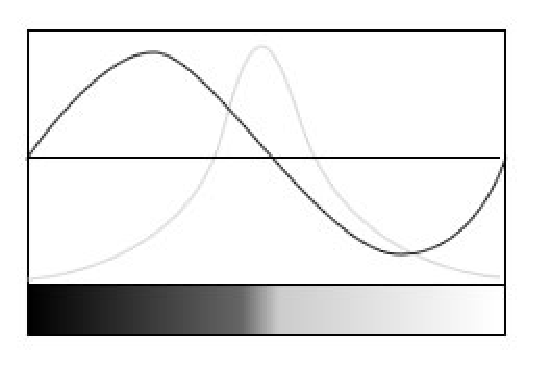
\includegraphics[width=0.5\textwidth]{eps_pics/sample-edge-second-derivative}
\caption{Second derivative of the curve in Figure \ref{fig:sobel_sample_edge}}
\label{fig:sobel_sample_edge_second_deriv}
}
\end{figure}

Since images are typically 2-D, a gradient is used to calculate the derivatives. Convolution kernels are used to approximate the gradients in the X and Y directions. These kernels are shown in Figure

\begin{figure}[ht!]
{
\centering
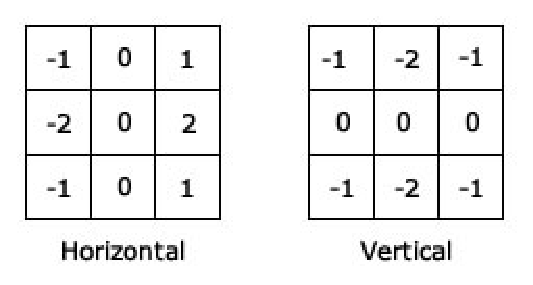
\includegraphics[width=0.5\textwidth]{eps_pics/sobel-kernels1.eps}
\caption{Convolution kernels}
\label{fig:sobel_kernels1}
}
\end{figure}

Can give the  magnitude:

\begin{equation}
\sqrt{G_x^2 + G_y^2}
\end{equation}

Approx strength:

\begin{equation}
|G_x| + |G_y|
\end{equation}

And the edge orientation:

\begin{equation}
arctan(\frac{G_y}{G_x})
\end{equation}